\documentclass[11pt,a4paper]{article}

\usepackage[margin=2.4cm]{geometry}
\usepackage{xcolor}
\usepackage{tikz}
\usetikzlibrary{arrows.meta, positioning, shapes.geometric, calc}
\usepackage{listings}
\usepackage{booktabs}
\usepackage{tabularx}
\usepackage{array}
\usepackage{amsmath}
\usepackage{graphicx}
\usepackage{fancyhdr}
\usepackage{titlesec}
\usepackage{enumitem}
\usepackage{microtype}
\usepackage[hidelinks]{hyperref}

\definecolor{ferblue}{HTML}{1F4E79}
\definecolor{fermaroon}{HTML}{7B2D26}
\definecolor{fergray}{HTML}{5A5A5A}
\definecolor{ferlight}{HTML}{EEF3F8}

\titleformat{\section}{\Large\bfseries\color{ferblue}}{\thesection}{0.8em}{}
\titleformat{\subsection}{\large\bfseries\color{ferblue!80}}{\thesubsection}{0.7em}{}

\pagestyle{fancy}
\fancyhf{}
\fancyhead[L]{\small\color{fergray}Ferrite --- Technical Guide}
\fancyhead[R]{\small\color{fergray}\thepage}
\renewcommand{\headrulewidth}{0.4pt}


\lstdefinestyle{cstyle}{
  language=C,
  basicstyle=\ttfamily\footnotesize,
  keywordstyle=\color{ferblue}\bfseries,
  commentstyle=\color{fergray}\itshape,
  stringstyle=\color{fermaroon},
  numbers=left, numberstyle=\tiny\color{fergray},
  numbersep=6pt,
  frame=single, rulecolor=\color{fergray!40},
  framesep=4pt, xleftmargin=16pt,
  breaklines=true,
  showstringspaces=false,
  morekeywords={FeStatus, FeTensor, FeArena, FeGraph, FeNode, FeTensorEntry,
    FeRuntime, FePlan, FeProfiler, FeQuantParams, FeOpType, FeDtype,
    __m256, uint32_t, uint64_t, int32_t, int8_t, size_t, uintptr_t},
}

\setcounter{tocdepth}{2}
\setlength{\parskip}{4pt}

\begin{document}

\begin{titlepage}
\centering
\vspace*{2.5cm}
{\Huge\bfseries\color{ferblue} Ferrite\par}
\vspace{0.4cm}
{\LARGE A Zero-Dependency Neural-Network Inference Runtime in C11\par}
\vspace{1.2cm}
{\large Technical Guide --- Subsystems, Algorithms, and Design Decisions\par}
\vspace{2.2cm}

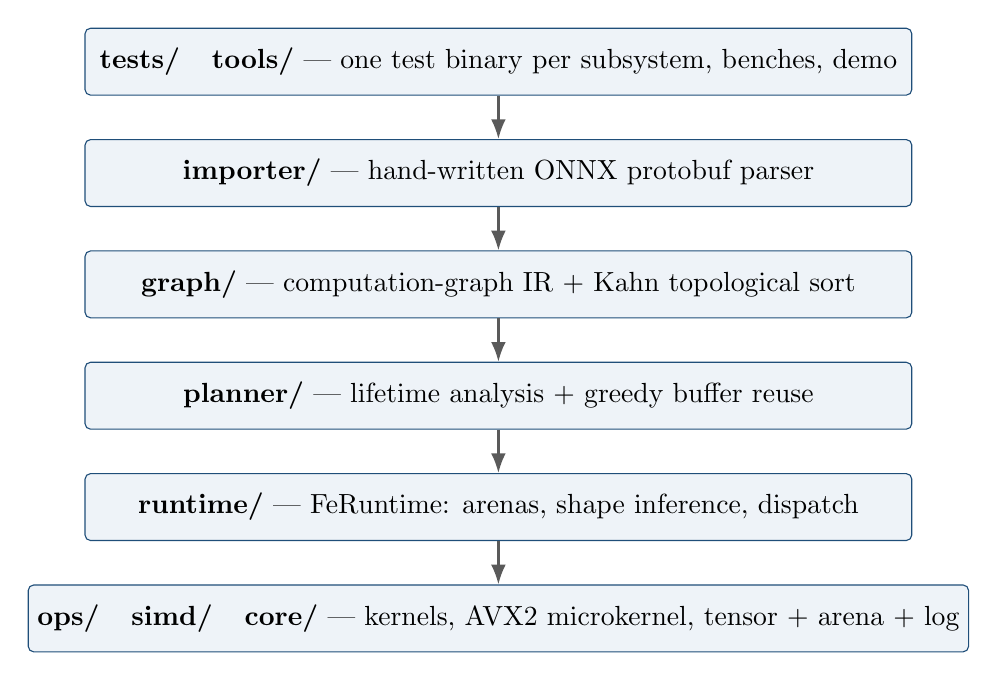
\begin{tikzpicture}[node distance=0.55cm,
  layer/.style={rectangle, rounded corners=2pt, draw=ferblue, fill=ferlight,
                minimum width=10.5cm, minimum height=0.85cm, align=center},
  arr/.style={-{Latex[length=2.5mm]}, thick, fergray}]
  \node[layer] (tests) {\textbf{tests/ \ \ tools/} --- one test binary per subsystem, benches, demo};
  \node[layer, below=of tests] (importer) {\textbf{importer/} --- hand-written ONNX protobuf parser};
  \node[layer, below=of importer] (graph) {\textbf{graph/} --- computation-graph IR + Kahn topological sort};
  \node[layer, below=of graph] (planner) {\textbf{planner/} --- lifetime analysis + greedy buffer reuse};
  \node[layer, below=of planner] (runtime) {\textbf{runtime/} --- FeRuntime: arenas, shape inference, dispatch};
  \node[layer, below=of runtime] (kernels)
       {\textbf{ops/ \ \ simd/ \ \ core/} --- kernels, AVX2 microkernel, tensor + arena + log};
  \draw[arr] (tests) -- (importer);
  \draw[arr] (importer) -- (graph);
  \draw[arr] (graph) -- (planner);
  \draw[arr] (planner) -- (runtime);
  \draw[arr] (runtime) -- (kernels);
\end{tikzpicture}

\vfill
{\large Generated from source by \texttt{temps/build\_guide.py} \par}
{\color{fergray}\today\par}
\end{titlepage}

\tableofcontents
\newpage

\section{What Ferrite Is}

Ferrite loads ONNX neural-network models and executes them on the CPU using
hand-written C11 kernels. It has \textbf{zero external dependencies}: no BLAS,
no protobuf library, no SIMD wrapper, no framework. Every mechanism it needs ---
strided tensors, an arena allocator, a protobuf wire parser, a topological sort,
a greedy memory planner, an AVX2 matrix-multiply microkernel --- is implemented
from first principles in this repository.

Three commitments shape every subsystem:

\begin{enumerate}[itemsep=2pt]
\item \textbf{One subsystem per commit.} The git history reads as a tour of the
      architecture; each subsystem landed with its own test binary.
\item \textbf{Correctness before speed.} The naive scalar \texttt{fe\_matmul} is the
      reference oracle. The AVX2 kernel must match it before it earns its place.
\item \textbf{Fail loudly, never silently.} Public functions return a
      \texttt{FeStatus} code; unsupported operations produce errors, not guesses.
\end{enumerate}

\subsection{Layer Rule}

Dependencies point strictly downward (Figure on the title page):
\[
\texttt{importer} \rightarrow \texttt{graph} \rightarrow \texttt{planner}
\rightarrow \texttt{runtime} \rightarrow \texttt{ops} + \texttt{simd} +
\texttt{core}
\]
with \texttt{tests/} and \texttt{tools/} sitting on top of everything. No upper
layer may be included by a lower one; the CMake static libraries enforce this
at link time.

\subsection{Repository Map}

\begin{tabularx}{0.94\textwidth}{@{}l X@{}}
\toprule
\textbf{File(s)} & \textbf{Role} \\
\midrule
core/types.h & FeDtype, FeStatus enums, fe\_dtype\_size, FERRITE\_MAX\_DIMS=8 \\
core/tensor.c/h & FeTensor strided views: alloc/slice/transpose/reshape/contiguous/copy; stride-0 broadcast\_to; numel; get/set\_f32; allclose \\
core/tensor\_ser.c/h & versioned binary serialization (FETN v1), strict validating reader \\
core/allocator.c/h & FeArena bump allocator; pointer-address alignment; peak tracking \\
core/log.c/h & fe\_log level-filtered stderr logging (compile-time minimum) \\
graph/graph.c/h & fixed-capacity IR: nodes, tensor registry, Kahn topological sort \\
ops/matmul.c & i-k-j scalar reference + AVX2 dispatch behind CPUID gate; fe\_linear wrapper \\
ops/activations.c & relu, last-axis stable softmax (inv-sum third pass), broadcast bias\_add \\
ops/elementwise.c & fe\_add/sub/mul/div + scalar variants + fe\_neg; exact-shape fp32 flat loops \\
ops/reduce.c & single-axis fe\_sum/fe\_max/fe\_min with axis-removed output; rank-1 fe\_dot \\
ops/stability.c & max-shift fe\_logsumexp and fe\_stable\_exp\_normalize (1-D fp32, two passes) \\
ops/conv1d.c & im2col transformation + matmul; per-call scratch buffer \\
simd/matmul\_avx2.c/h & tiled AVX2+FMA microkernel; CPUID detection; remainder columns \\
planner/memory\_planner.c/h & lifetime analysis + greedy best-fit buffer reuse; FePlan offsets \\
runtime/engine.c/h & FeRuntime lifecycle, shape inference, dispatch walk, output copy \\
importer/onnx.c & hand-written protobuf wire parser -$>$ graph build -$>$ weights to arena \\
quantization/quant.c & symmetric INT8 per-tensor quantize/dequantize + int8 GEMM path \\
tools/profiler.c & per-op ns timing records, CLOCK\_MONOTONIC, sorted report \\
tools/bench\_matmul.c & naive GFLOPS at N=256 over 20 runs \\
tools/bench\_avx2.c & AVX2 vs naive GFLOPS, correctness verify, speedup print \\
tools/demo\_acousticleaknet.c & end-to-end demo: acoustic leak-detection CNN on synthetic audio \\
\bottomrule
\end{tabularx}

\section{Core Data Structures (\texttt{core/})}

\subsection{The Strided Tensor --- \texttt{FeTensor}}

The tensor is the universal currency of the runtime: graphs move tensors,
kernels consume tensors, the planner places tensors. Everything hinges on one
plain struct:

\begin{lstlisting}[style=cstyle,caption={core/tensor.h --- the entire tensor abstraction}]
typedef struct {
    void    *data;
    FeDtype  dtype;
    int      ndim;
    int      shape  [FERRITE_MAX_DIMS];   /* logical extent per axis */
    int      strides[FERRITE_MAX_DIMS];  /* IN ELEMENTS, not bytes  */
    size_t   nbytes;
    bool     owns_data;
} FeTensor;
\end{lstlisting}

Design rule: \emph{metadata over behavior}. The struct computes nothing and
stores everything. All shape operations --- transpose, reshape, slice ---
manipulate these fields only, which is what makes views free:

\begin{itemize}[itemsep=2pt]
\item \textbf{Transpose} swaps two axes' \texttt{shape} and \texttt{stride}
      entries. O(1), zero data movement.
\item \textbf{Slice} shifts \texttt{data} forward by
      $start \times strides[axis] \times elem\_size$ bytes and shrinks one axis.
      Strides stay untouched --- that is the whole trick.
\item \textbf{Reshape} succeeds \emph{only} on contiguous tensors and returns a
      view; element count must be preserved. Non-contiguous reshape is refused
      rather than silently copied.
\item \textbf{Contiguous repack} walks multi-dimensional indices and copies each
      element to its packed position. This is the bridge from ``any layout'' to
      ``what kernels require.''
\end{itemize}

\paragraph{Worked example.} A $3\times4$ float32 tensor allocates 48 bytes.
Row-major strides are $\{4,1\}$: element $(i,j)$ lives at flat offset
$4i + j$. Transposing yields a $4\times3$ \emph{view} with strides $\{1,4\}$ ---
same buffer, different interpretation (Figure~\ref{fig:strides}).

\begin{figure}[h]
\centering
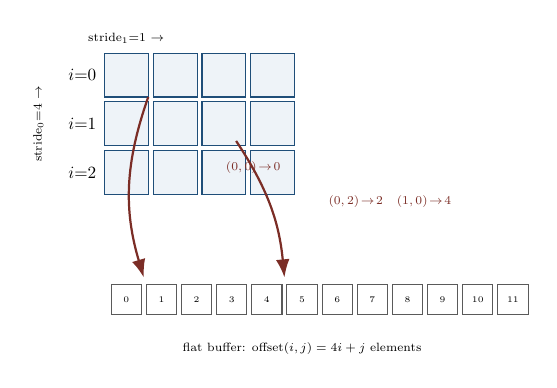
\begin{tikzpicture}[scale=0.62, every node/.style={transform shape}]
  % logical grid
  \foreach \i in {0,...,2}
    \foreach \j in {0,...,3}
      \node[draw=ferblue, fill=ferlight, minimum size=0.9cm] at (\j,-\i) {};
  \foreach \i/\j/\v in {0/0/{(0,0)}, 1/0/{(0,1)}, 2/0/{(0,2)}} {}
  \node at (-0.9,0) {$i{=}0$};
  \node at (-0.9,-1) {$i{=}1$};
  \node at (-0.9,-2) {$i{=}2$};
  \node at (0,0.75) {\scriptsize stride$_1{=}1$ $\rightarrow$};
  \node[rotate=90] at (-1.8,-1) {\scriptsize stride$_0{=}4$ $\rightarrow$};
  % flat buffer
  \foreach \k in {0,...,11}
    \node[draw=fergray, fill=white, minimum size=0.62cm] at (\k*0.72,-4.6) {\tiny\k};
  \node at (3.6,-5.6) {\scriptsize flat buffer: offset$(i,j) = 4i+j$ elements};
  \draw[-{Latex}, thick, fermaroon] (0.45,-0.45) to[bend right=18] (0.36,-4.15);
  \node[fermaroon] at (2.6,-1.9) {\scriptsize $(0,0)\!\to\!0$};
  \draw[-{Latex}, thick, fermaroon] (2.25,-1.35) to[bend left=14] (3.24,-4.15);
  \node[fermaroon] at (5.4,-2.6) {\scriptsize $(0,2)\!\to\!2$\ \ \ $(1,0)\!\to\!4$};
\end{tikzpicture}
\caption{Row-major layout. Strides turn address arithmetic into pure metadata:
no copy ever moves between the grid view and the flat buffer.}
\label{fig:strides}
\end{figure}

\paragraph{Ownership.} One invariant rules memory safety:
\texttt{owns\_data == true} frees the buffer inside \texttt{fe\_tensor\_free()};
views never free their parent's. Arena-produced tensors set
\texttt{owns\_data=false} permanently --- passing one to \texttt{fe\_tensor\_free}
would corrupt the arena, and the header warns against exactly that.


\subsection{Slicing --- \texttt{fe\_tensor\_slice}}

A second wave of view factories (``Stage 1'' in the roadmap) rounds out the
tensor abstraction so the math backend can operate on sub-ranges without ever
copying. Slicing takes \texttt{(axis, start, len)} and walks a pure metadata
path:

\begin{lstlisting}[style=cstyle,caption={core/tensor.c --- slicing is three lines of arithmetic}]
FeTensor *fe_tensor_slice(const FeTensor *t, int axis, int start, int len) {
    assert(axis >= 0 && axis < t->ndim);
    assert(start >= 0 && len > 0 && start + len <= t->shape[axis]);

    FeTensor *view = calloc(1, sizeof(FeTensor));
    if (!view) return NULL;

    *view = *t;                      /* copy everything: dtype, strides, ndim */
    view->owns_data = false;         /* a view never owns memory */
    view->shape[axis] = len;         /* only this axis shrinks */

    size_t elem = fe_dtype_size(t->dtype);
    view->data = (char *)t->data
               + (size_t)start * (size_t)t->strides[axis] * elem;

    view->nbytes = elem;             /* recount bytes for the smaller shape */
    for (int i = 0; i < view->ndim; i++) view->nbytes *= (size_t)view->shape[i];
    return view;
}
\end{lstlisting}

The API is deliberately \texttt{(axis, start, len)} rather than a general
\emph{starts/ends/step} triple: one axis, no reverse strides, every bound
checked by assertion. The whole trick is that \texttt{strides} are untouched ---
advancing along the sliced axis still costs \texttt{strides[axis]} elements, so
the view's \emph{extent} shrinks while its \emph{geometry} is inherited from the
parent. The data pointer moves by exactly
$start \times strides[axis] \times elem\_size$ elements. In
\texttt{test\_tensor}, slicing the $4\times3$ grid at
\texttt{(axis=0, start=1, len=2)} yields a view whose element \texttt{\{0,0\}}
is the parent's \texttt{\{1,0\}} (value 3.0) and whose \texttt{\{1,2\}} is the
parent's \texttt{\{2,2\}} (value 8.0) --- both verified through
\texttt{fe\_tensor\_get\_f32}, proving the pointer shift happened in element
space, not byte space.

\subsection{Broadcasting --- Stride-Zero Views}

\emph{Normalization} broadcasting is a pure metadata trick: a matrix of 4 rows
multiplied by a vector of 3 entries can reuse the same three floats for every
row if the row axis has stride 0. \texttt{fe\_tensor\_broadcast\_to} builds
exactly that view, NumPy-style, aligning the \emph{trailing} axes:

\begin{lstlisting}[style=cstyle,caption={core/tensor.c --- stride-0 broadcasting, back-aligned}]
FeTensor *fe_tensor_broadcast_to(const FeTensor *t, int ndim,
                                 const int *target_shape) {
    assert(ndim >= t->ndim);         /* can only broadcast to equal/more dims */

    FeTensor *view = calloc(1, sizeof(FeTensor));
    if (!view) return NULL;

    *view = *t;
    view->owns_data = false;
    view->ndim = ndim;

    int diff = ndim - t->ndim;       /* leading dims t is missing */

    for (int i = ndim - 1; i >= 0; i--) {
        int t_axis = i - diff;
        int t_size = (t_axis >= 0) ? t->shape[t_axis] : 1;

        view->shape[i] = target_shape[i];

        if (t_size == target_shape[i]) {
            /* Sizes match: keep the real stride (0 if the axis is synthetic) */
            view->strides[i] = (t_axis >= 0) ? t->strides[t_axis] : 0;
        } else if (t_size == 1) {
            view->strides[i] = 0;    /* size-1 axis: reuse one element forever */
        } else {
            free(view);              /* incompatible shapes: refuse, not guess */
            return NULL;
        }
    }
    return view;
}
\end{lstlisting}

Three cases drive the backward walk. A synthetic leading axis (the source has no
axis there) collapses to stride 0 --- reading the tensor ``along'' that axis
always hits element 0. A real axis whose size matches the target keeps its
parent stride, so the view reuses genuine memory. A real \emph{size-1} axis
broadcasts by zeroing its stride. Anything else is a shape conflict and the view
is freed --- returning \texttt{NULL}, never a copy.

\begin{figure}[h]
\centering
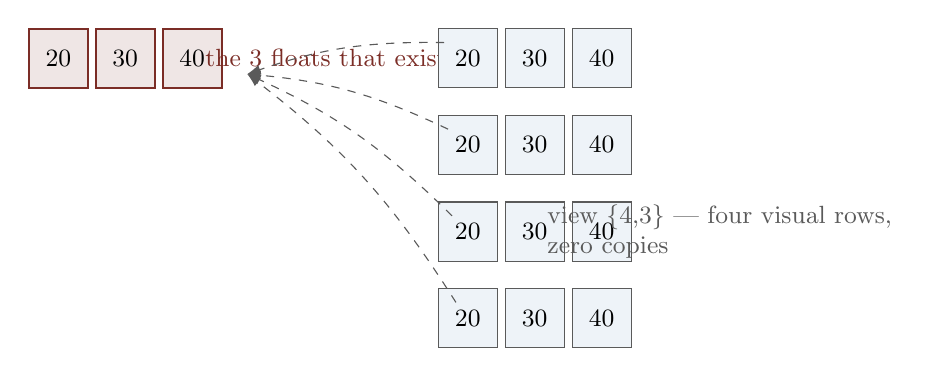
\begin{tikzpicture}[every node/.style={font=\small}]
  % physical storage: the one and only row
  \foreach \v/\x in {20/0,30/1,40/2}
    \node[draw=fermaroon, thick, fill=fermaroon!12, minimum size=0.75cm] at (\x*0.85,0) {\v};
  \node[fermaroon] at (3.4,-0.0) {the $3$ floats that exist};
  % the broadcast view: 4 rows, all pointing at the same storage
  \foreach \r in {0,...,3} {
    \foreach \v/\x in {20/0,30/1,40/2}
      \node[draw=fergray, fill=ferlight, minimum size=0.75cm] at (5.2+\x*0.85,-1.1*\r) {\v};
    \draw[-{Latex}, dashed, fergray] (4.9+\r*0.05,-1.1*\r+0.2) to[bend right=10] (2.4,-0.2);
  }
  \node[fergray, align=left] at (8.4,-2.2) {view \{4,3\} --- four visual rows,\\ zero copies};
\end{tikzpicture}
\caption{Broadcast to \{4,3\}: the row axis gets \texttt{strides[0] = 0}, so
every ``row'' of the view reads the same three floats. Cost of broadcasting:
three integers in the metadata, not twelve floats in memory.}
\label{fig:bcast}
\end{figure}

The elem-walk must respect these views: index \texttt{\{r, c\}} computes
$r\cdot 0 + c\cdot 1 = c$, and that is exactly what \texttt{fe\_tensor\_get\_f32}
does (next subsection). \texttt{test\_tensor} locks the behavior
\emph{structurally}: broadcasting \{1,3\} to \{4,3\} must yield
\texttt{shape=\{4,3\}}, \texttt{strides[0]==0}, \texttt{strides[1]} unchanged,
and \texttt{fe\_tensor\_get\_f32(b, \{row,1\})==20.0} for \emph{every} row.

\subsection{Element Access and Comparison Helpers}

\texttt{fe\_tensor\_get\_f32} / \texttt{fe\_tensor\_set\_f32} are the strided
element primitives --- declared \emph{for testing and debugging, never the hot
path}. Both fold a multi-index into a flat offset via the stride table:

\begin{lstlisting}[style=cstyle,caption={core/tensor.c --- strided element access}]
float fe_tensor_get_f32(const FeTensor *t, const int *idx) {
    size_t off = 0;
    for (int d = 0; d < t->ndim; d++) off += (size_t)idx[d] * t->strides[d];
    return ((const float *)t->data)[off];
}

/* The odometer: +1 on the rightmost axle, carrying left like base-N counting */
int idx[FERRITE_MAX_DIMS] = {0};
for (int i = 0; i < fe_tensor_numel(t); i++) {
    /* ... visit t at index idx ... */
    for (int d = t->ndim - 1; d >= 0; d--) {
        if (++idx[d] < t->shape[d]) break;
        idx[d] = 0;
    }
}
\end{lstlisting}

The odometer increment --- \emph{increment the last axle; if it overflows,
reset it and carry to the previous axle} --- is the multi-dimensional counter
used by four sites in the tree (\texttt{fe\_tensor\_contiguous},
\texttt{fe\_tensor\_copy}, \texttt{fe\_tensor\_allclose}, and the reduction
kernel in \texttt{ops/reduce.c}). It trades a tiny bit of recomputation for
total shape generality: no fixed strip pattern, just ndim and a stride table.

\texttt{fe\_tensor\_allclose(a, b, tol)} is the comparison primitive: shapes must
match exactly, dtypes must match \emph{and} be float32, then every element pair
is compared with \texttt{fabsf(va - vb) \(\le\) tol}. It exists because
reordered arithmetic is never bit-identical: tests that would be brittle under
\texttt{==} assert against \texttt{allclose} instead. \texttt{test\_tensor}
proves the tolerance contract: \texttt{a[i]=i} vs \texttt{b[i]=i+0.0001} is
\emph{true} at tol 0.001 and \emph{false} at tol 0.00001.
\subsection{The Arena Allocator --- \texttt{FeArena}}

A bump allocator: allocation advances one pointer, reset rewinds it. O(1) alloc,
all-or-nothing free.

\begin{lstlisting}[style=cstyle,caption={core/allocator.c --- alignment happens on the real pointer}]
uintptr_t current = (uintptr_t)(a->base + a->offset);
uintptr_t aligned = (current + align - 1) & ~(uintptr_t)(align - 1);
size_t new_offset = aligned - (uintptr_t)a->base + size;
if (new_offset > a->size) return NULL;          /* exhausted */
a->offset = new_offset;
if (a->offset > a->peak) a->peak = a->offset;   /* high-water mark */
\end{lstlisting}

Subtleties worth naming:

\begin{itemize}[itemsep=2pt]
\item Alignment masks the \emph{actual pointer address}, not merely the stored
      offset --- they differ whenever \texttt{base} itself is unaligned.
\item \texttt{fe\_arena\_reset} keeps \texttt{peak} on purpose: after thousands
      of inference calls, peak \emph{is} the true memory-footprint number.
\item \texttt{fe\_arena\_alloc\_tensor} allocates metadata and payload together,
      payload at literal 64-byte alignment for AVX2 load/store efficiency, and
      computes row-major strides eagerly.
\item The intended split: a \textbf{weight arena} allocated once at model load
      and never reset; an \textbf{activation arena} reset every inference call.
      This is the classic inference-runtime memory strategy.
\end{itemize}

\subsection{Shared Types --- Dtypes and Status Codes}

\texttt{fe\_dtype\_size} is the single source of truth for element width; every
kernel validates dtype through it before touching data.

\begin{table}[h]
\centering
\begin{tabular}{@{}llll@{}}
\toprule
\textbf{Enum value} & \textbf{Id} & \textbf{Bytes} & \textbf{Where used} \\
\midrule
DTYPE\_FLOAT32 & 0 & 4 & every kernel; the only dtype kernels accept today\\
DTYPE\_INT8 & 1 & 1 & quantization storage (symmetric per-tensor)\\
DTYPE\_INT32 & 2 & 4 & int8 GEMM accumulation target\\
\bottomrule
\end{tabular}
\caption{The dtype table. Adding float64 later means one enum entry and one
size entry --- every consumer already routes through \texttt{fe\_dtype\_size}.}
\end{table}

\begin{table}[h]
\centering
\small
\begin{tabularx}{\textwidth}{@{}ll X@{}}
\toprule
\textbf{Code} & \textbf{Value} & \textbf{Meaning} \\
\midrule
FE\_OK & 0 & full success; all outputs written\\
FE\_ERR\_NULL & 1 & required pointer argument was NULL\\
FE\_ERR\_SHAPE & 2 & shape/rank mismatch or unsupported shape; also the engine's ``unimplemented op'' signal\\
FE\_ERR\_DTYPE & 3 & dtype mismatch, unknown, or unsupported\\
FE\_ERR\_NOMEM & 4 & allocation failed\\
FE\_ERR\_BOUNDS & 5 & index out of range\\
FE\_ERR\_IO & 6 & file open/read/write/format failure (added for serialization)\\
\bottomrule
\end{tabularx}
\caption{FeStatus contract. FE\_OK means full success with all outputs written;
on error callees never free caller memory nor partially mutate outputs.}
\end{table}

\subsection{Logging --- \texttt{core/log.h}}

Four levels (DEBUG/INFO/WARN/ERROR) write \texttt{[ferrite LEVEL file:line] msg}
to stderr. \texttt{FERRITE\_LOG\_LEVEL} sets the compile-time floor: filtered
calls expand to \texttt{((void)0)} and vanish. Default is WARN. Policy: import
and init boundaries log; \textbf{kernels never log} --- no I/O in hot paths.
(The one current violator, a debug trace in \texttt{fe\_conv1d}, is flagged in
\S\ref{sec:honest}.)

\section{Tensor Serialization --- \texttt{core/tensor\_ser}}

Tensors round-trip to disk through a versioned binary format. The guiding
decision: \emph{serialize the logical contents, not the struct}. Strides,
pointers, and ownership flags are layout details of the running process and
mean nothing on disk.

\begin{table}[h]
\centering
\begin{tabular}{@{}clll@{}}
\toprule
\textbf{Offset} & \textbf{Size} & \textbf{Field} & \textbf{Notes} \\
\midrule
0 & 4 & magic \texttt{"FETN"} & rejects non-Ferrite files immediately \\
4 & 4 & version (u32) & currently 1; readers reject anything newer \\
8 & 4 & dtype (u32) & validated via \texttt{fe\_dtype\_size} \\
12 & 4 & ndim (u32) & must be 1..8 ($\le$ \texttt{FERRITE\_MAX\_DIMS}) \\
16 & $4n$ & shape[] (i32) & every axis $\ge 1$ \\
$16{+}4n$ & 8 & data\_len (u64) & must equal computed byte count \\
$24{+}4n$ & $n$ & payload & raw row-major element bytes \\
\bottomrule
\end{tabular}
\caption{FETN v1 layout. All integers are little-endian on every host ---
written through explicit byte-shuffling helpers, not raw struct dumps.}
\end{table}

\paragraph{Views save canonically.} Saving a transposed view first repacks it
through \texttt{fe\_tensor\_contiguous()}, reusing the tested repack walk instead
of duplicating it. Loading always produces a fresh owning, row-major tensor.

\paragraph{The reader trusts nothing.} Wrong magic, future version, unknown
dtype, impossible rank, zero axes, a \texttt{data\_len} that disagrees with the
computed count, truncated payloads, trailing garbage --- each maps to a specific
error (\texttt{FE\_ERR\_IO/DTYPE/SHAPE}), and every failure path frees partial
state before returning. Strictness is deliberate: within v1 even one extra
trailing byte is corruption. Version rejection is the forward-compatibility
seam --- v2 may change anything, because old builds refuse to guess.

\begin{lstlisting}[style=cstyle,caption={tests/test\_tensor\_ser.c --- one-byte mutations, one assertion each}]
#define MUTATE(off, b)                        \
    do {                                      \
        write_valid_minimal(TMP_A);           \
        FILE *mf = fopen(TMP_A, "r+b");       \
        fseek(mf, (off), SEEK_SET);           \
        fputc((b), mf);                       \
        fclose(mf);                           \
    } while (0)

MUTATE(8, 77);   /* unknown dtype            */
assert(fe_tensor_load(TMP_A, &out) == FE_ERR_DTYPE);
\end{lstlisting}

\section{Computation Graph --- \texttt{graph/}}

The IR separates structure from data. At build time a tensor is pure metadata;
actual pointers appear only when the runtime assigns them.

\begin{lstlisting}[style=cstyle,caption={graph/graph.h --- fixed-capacity IR}]
#define FE_MAX_NODES   512
#define FE_MAX_TENSORS 1024

typedef struct {
    char     name[64];
    FeOpType op;
    int      inputs [FE_MAX_NODE_INPUTS];   /* INDICES into tensors[] */
    int      outputs[FE_MAX_NODE_OUTPUTS];
    union { struct { int axis; } softmax;
            struct { int stride, pad; } conv1d; } attrs;
} FeNode;

typedef struct {
    char      name[64];
    int       shape[FERRITE_MAX_DIMS];
    int       ndim;  FeDtype dtype;
    FeTensor *tensor;      /* NULL until memory is assigned */
    int       is_weight;
} FeTensorEntry;
\end{lstlisting}

Nodes reference tensors \textbf{by index}, never by pointer. Indices survive
reallocation-free fixed arrays, serialize trivially, and cannot dangle.
Capacities are hard limits (512 nodes / 1024 tensors / 8 dims) --- embedded-style
predictability over dynamic growth. Adding any node invalidates a previous sort
(\texttt{topo\_valid = 0}), forcing re-planning.

\subsection{Kahn Topological Sort, Step by Step}

\begin{enumerate}[itemsep=2pt]
\item Build a producer map: for every node, mark each output tensor with that
      node's id (weights and external inputs have producer $-1$).
\item Count in-degrees: each node gains one edge per input whose producer
      exists --- so weights contribute nothing.
\item Seed an array queue with all in-degree-zero nodes.
\item Pop, append to \texttt{topo\_order}, decrement every consumer's in-degree;
      zeros enqueue. (The consumer scan walks all nodes' input lists --- honest
      $O(N \cdot E)$, though the doc comment claims $O(N+E)$; fine at $N \le 512$.)
\item If fewer nodes were emitted than exist, a cycle traps the remainder:
      return \texttt{FE\_ERR\_SHAPE}.
\end{enumerate}

\begin{figure}[h]
\centering
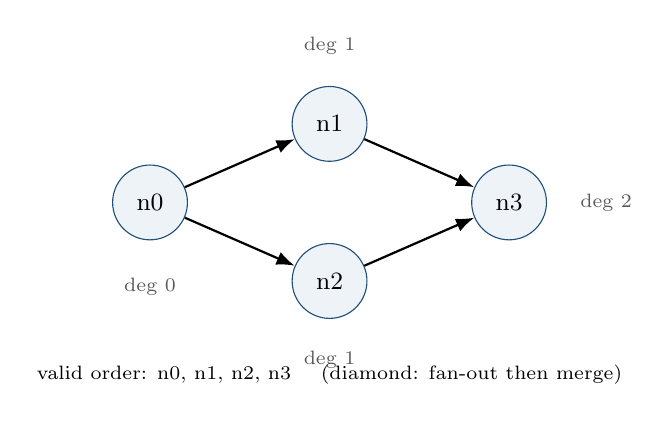
\begin{tikzpicture}[scale=0.95, node distance=1.5cm,
  n/.style={circle, draw=ferblue, fill=ferlight, minimum size=0.95cm, font=\small}]
  \node[n] (n0) at (0,0) {n0};
  \node[n] (n1) at (2.4,1.05) {n1};
  \node[n] (n2) at (2.4,-1.05) {n2};
  \node[n] (n3) at (4.8,0) {n3};
  \draw[-{Latex}, thick] (n0) -- (n1);
  \draw[-{Latex}, thick] (n0) -- (n2);
  \draw[-{Latex}, thick] (n1) -- (n3);
  \draw[-{Latex}, thick] (n2) -- (n3);
  \node[below=0.35cm of n0, font=\scriptsize\color{fergray}] {deg 0};
  \node[above=0.28cm of n1, font=\scriptsize\color{fergray}] {deg 1};
  \node[below=0.28cm of n2, font=\scriptsize\color{fergray}] {deg 1};
  \node[right=0.3cm of n3, font=\scriptsize\color{fergray}] {deg 2};
  \node[font=\scriptsize] at (2.4,-2.3)
      {valid order: n0, n1, n2, n3 \quad (diamond: fan-out then merge)};
\end{tikzpicture}
\caption{The diamond graph from \texttt{test\_graph}: n0 fans out to n1/n2,
which merge into n3. Kahn's algorithm emits n0 first and n3 last --- the exact
assertion the test makes.}
\label{fig:diamond}
\end{figure}

\section{Operator Kernels --- \texttt{ops/}}

Every kernel obeys one contract: \textbf{inputs read-only, output
caller-allocated with correct shape, no allocation inside, validate
pointers/dtypes/shapes before touching data.} This makes kernels composable and
makes the planner possible --- nobody but the caller decides where results land.

\subsection{Matrix Multiply and Its Dispatch}

The naive reference is an \emph{i-k-j} loop --- the innermost statement slides
contiguously along B's rows and C's rows, so each cache line fetched does full
work:

\begin{lstlisting}[style=cstyle]
for (int i = 0; i < M; i++)
  for (int k = 0; k < K; k++) {
    float a_ik = a[i*K + k];
    for (int j = 0; j < N; j++)
      c[i*N + j] += a_ik * b[k*N + j];
  }
\end{lstlisting}

\texttt{fe\_matmul} itself is now a dispatcher: probe \texttt{fe\_cpu\_has\_avx2()},
try the SIMD kernel, fall back to scalar on any failure. The naive loop remains
the correctness oracle regardless (\S\ref{sec:simd}). \texttt{fe\_linear} composes
two primitives: \texttt{fe\_matmul(A,W,C)} followed by an in-place
\texttt{fe\_bias\_add(C,b,C)}.

\subsection{Softmax Without Explosions}

Numerically stable last-axis softmax: subtract the row maximum before
exponentiating.
\[
\mathrm{softmax}(x)_c = \frac{e^{x_c - m}}{\sum_{c'} e^{x_{c'} - m}},
\qquad m = \max_c x_c
\]
Mathematically identical, but $e^{x_c-m} \le 1$, so \texttt{expf} can never
overflow to infinity. \texttt{test\_ops} feeds it $\{1000, 1001, 1002\}$ ---
unstable implementations produce NaN there.

\texttt{fe\_bias\_add} broadcasts one bias vector across leading dimensions:
with \texttt{cols = shape[ndim-1]}, element $(r, c)$ gains \texttt{b[c]}. The
engine exploits this for ONNX \texttt{Add}: broadcasting a same-shaped input
degenerates into exactly this loop.


\subsection{Elementwise Arithmetic --- 9 Ops, One Shape Rule}

The Stage 2 math backend adds the arithmetic layer: four vectorized binary
operators, their four scalar twins, and negation. All nine share two private
kernels and one validation law.

\begin{lstlisting}[style=cstyle,caption={ops/elementwise.c --- the binary kernel}]
typedef enum { OP_ADD, OP_SUB, OP_MUL, OP_DIV } ElemOp;
typedef enum { SOP_ADD, SOP_SUB, SOP_MUL, SOP_DIV } ScalarOp;

static FeStatus elementwise_binary(const FeTensor *a, const FeTensor *b,
                                   FeTensor *out, ElemOp op) {
    if (!a || !b || !out)                     return FE_ERR_NULL;
    if (a->ndim != b->ndim || a->ndim != out->ndim)  return FE_ERR_SHAPE;
    for (int i = 0; i < a->ndim; i++)
        if (a->shape[i] != b->shape[i] || a->shape[i] != out->shape[i])
            return FE_ERR_SHAPE;              /* exact shape equality */
    if (a->dtype != DTYPE_FLOAT32 || b->dtype != DTYPE_FLOAT32 ||
        out->dtype != DTYPE_FLOAT32)          return FE_ERR_DTYPE;

    int n = fe_tensor_numel(a);
    const float *pa = (const float *)a->data;
    const float *pb = (const float *)b->data;
    float       *po = (float *)out->data;

    switch (op) {
        case OP_ADD: for (int i = 0; i < n; i++) po[i] = pa[i] + pb[i]; break;
        case OP_SUB: for (int i = 0; i < n; i++) po[i] = pa[i] - pb[i]; break;
        case OP_MUL: for (int i = 0; i < n; i++) po[i] = pa[i] * pb[i]; break;
        case OP_DIV: for (int i = 0; i < n; i++) po[i] = pa[i] / pb[i]; break;
    }
    return FE_OK;
}
\end{lstlisting}

The public surface is a thin switch over that kernel plus a scalar sibling
(\texttt{scalar\_binary}: same validation, one operand hoisted into a
\texttt{float scalar}):

\[
\begin{array}{llll}
\texttt{fe\_add(a,b,o)} & \texttt{fe\_sub(a,b,o)} & \texttt{fe\_mul(a,b,o)} & \texttt{fe\_div(a,b,o)} \\
\texttt{fe\_add\_scalar(a,s,o)} & \texttt{fe\_sub\_scalar(a,s,o)} & \texttt{fe\_mul\_scalar(a,s,o)} & \texttt{fe\_div\_scalar(a,s,o)}\\
\multicolumn{4}{c}{\texttt{fe\_neg(a,o) = fe\_mul\_scalar(a,~-1.0f,~o)}}
\end{array}
\]

Three design decisions deserve naming. \textbf{(1) The shape law is ``exact
equality,'' not broadcasting.} Broadcasting lives in the view layer --- the
stride-0 views built by \texttt{fe\_tensor\_broadcast\_to}; these kernels are
the fast path for buffers that
are ``already the same shape,'' so they index the flat payload directly
\texttt{(pa[i])} and never consult strides. \textbf{(2) fp32 only, enforced
before any read.} \textbf{(3) Negation reuses the scalar path} ---
\texttt{return scalar\_binary(a, -1.0f, out, SOP\_MUL);} ---
one line of API for free, documented in the source as ``negation is just
mul by -1.''

\paragraph{The contiguous assumption, honestly.} Because elements are walked as
\texttt{pa[i]}, a \emph{stride-0 broadcast view} fed to \texttt{fe\_add} reads
the wrong memory on its broadcast axes --- the two layers are incompatible by
construction. This is accepted: activation buffers inside the engine are
contiguous by design, and the stride-aware kernels (reduce, stability) cover
the view-shaped cases. Division by zero is not guarded: IEEE semantics
(\texttt{inf}/\texttt{NaN}) are the contract, matching the reference softmax
tests.

Exactness in the tests is byte-exact because no reordering happens:
\texttt{\{1,2,3,4\}} + ``all 2s'' gives out[0]==3.0 and out[3]==6.0,
\texttt{mul} gives 2.0 and 8.0, \texttt{div} gives 0.5 and 2.0; the scalar
path gives \texttt{mul\_scalar(a, 10)} $\to$ \{10, 30\} and \texttt{neg} $\to$
{-1, -3}.

\subsection{Reductions --- Sum, Max, Min over One Axis}

Reduction removes exactly one axis: output shape is the input shape with
\texttt{axis} deleted, and every remaining output position combines
\texttt{shape[axis]} input values. The kernel is an odometer over output
positions, with the reduced axis mapped back into input coordinates:

\begin{lstlisting}[style=cstyle,caption={ops/reduce.c --- axis-removal machinery}]
    int reduce_len = in->shape[axis];
    int out_numel  = fe_tensor_numel(out);
    int in_idx[FERRITE_MAX_DIMS]  = {0};
    int out_idx[FERRITE_MAX_DIMS] = {0};

    for (int o = 0; o < out_numel; o++) {
        int d = 0;                              /* remap out -> in coords */
        for (int i = 0; i < in->ndim; i++) {
            if (i == axis) { in_idx[i] = 0; continue; }
            in_idx[i] = out_idx[d++];
        }

        float acc = (op == RED_SUM) ? 0.0f
                  : (op == RED_MAX) ? -FLT_MAX
                  : FLT_MAX;                    /* the seed, per combine */

        for (int k = 0; k < reduce_len; k++) {
            in_idx[axis] = k;
            float v = fe_tensor_get_f32(in, in_idx);   /* strided read */
            if (op == RED_SUM) acc += v;
            else if (op == RED_MAX) acc = v > acc ? v : acc;
            else acc = v < acc ? v : acc;
        }
        fe_tensor_set_f32(out, out_idx, acc);

        for (int i = out->ndim - 1; i >= 0; i--) {  /* odometer carry */
            if (++out_idx[i] < out->shape[i]) break;
            out_idx[i] = 0;
        }
    }
\end{lstlisting}

The accumulator seeds encode each op's identity element: sum seeds
\texttt{0.0f}, max seeds \texttt{-FLT\_MAX} (so any real input wins), min seeds
\texttt{+FLT\_MAX}. Inputs are read through \texttt{fe\_tensor\_get\_f32}
\emph{strided} --- the only op family to do so alongside stability --- so
reduce is the one place where a broadcast view \emph{can} flow through
arithmetic correctly. Combining is strict: bigger-than wins for max, smaller
for min, plain float accumulation for sum (no Kahan; accepted for activation
statistics, and deterministic in this build).

\begin{figure}[h]
\centering
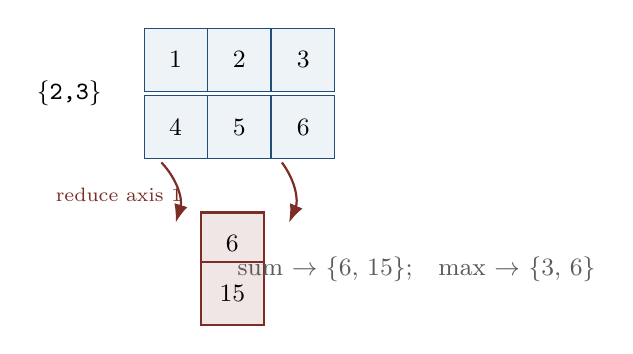
\begin{tikzpicture}[scale=0.9, every node/.style={font=\small}]
  % the {2,3} input
  \foreach \i/\v in {0/1,1/2,2/3}
    \node[draw=ferblue, fill=ferlight, minimum size=0.8cm] at (\i*0.9,0) {\v};
  \foreach \i/\v in {0/4,1/5,2/6}
    \node[draw=ferblue, fill=ferlight, minimum size=0.8cm] at (\i*0.9,-0.95) {\v};
  \node at (-1.5,-0.47) {\texttt{\{2,3\}}};
  % axis=1 collapse arrows
  \draw[-{Latex}, thick, fermaroon] (-0.2,-1.45) to[bend left=30] (0.0,-2.3);
  \draw[-{Latex}, thick, fermaroon] (1.5,-1.45) to[bend left=30] (1.6,-2.3);
  \node[fermaroon, font=\scriptsize] at (-0.8,-1.9) {reduce axis 1};
  % the {2} output
  \foreach \v/\y in {6/-2.6,15/-3.3}
    \node[draw=fermaroon, thick, fill=fermaroon!12, minimum size=0.8cm]
         at (0.8,\y) {\v};
  \node[fergray] at (3.4,-2.95) {sum $\to$ \{6, 15\};\quad max $\to$ \{3, 6\}};
\end{tikzpicture}
\caption{\texttt{fe\_sum} over the last axis of \{2,3\}: output shape \{2\};
each output cell combines its entire column. The test asserts 6, 15 for sum and
3, 6 for max --- both byte-exact.}
\label{fig:reduce}
\end{figure}

\texttt{fe\_dot} is the rank-1 cousin: \emph{not} a tensor output but a
\texttt{float *}. It requires both operands rank 1 with equal length, then
accumulates $a_i \cdot b_i$ through strided reads and stores the scalar. The
test {1,2,3} \textbullet {} {4,5,6} lands exactly on 32.0 ($4+10+18$).

\subsection{Numerical Stability --- the Max-Shift Identity}

Two new helpers attack the classic failure of Log-Sum-Exp and softmax:
\texttt{expf} with a large argument overflows to \texttt{inf}, poisoning the
sum and the ratio. The fix is the identity
\[
\operatorname{LSE}(x)=\log\sum_i e^{x_i}
=\ m+\log\sum_i e^{\,x_i-m},
\qquad m=\max_i x_i,
\]
which holds for any shift $m$ and makes every exponential argument $\le 0$ ---
so $e^{x_i-m}\le 1$, no overflow ever. \texttt{fe\_logsumexp} implements it in
two passes (find max, then accumulate shifted exponentials):

\begin{lstlisting}[style=cstyle,caption={ops/stability.c --- fe\_logsumexp, two passes over a 1-D vector}]
FeStatus fe_logsumexp(const FeTensor *in, float *out) {
    if (!in || !out) return FE_ERR_NULL;
    if (in->ndim != 1) return FE_ERR_SHAPE;
    if (in->dtype != DTYPE_FLOAT32) return FE_ERR_DTYPE;

    int n = in->shape[0];
    float max_val = -FLT_MAX;
    for (int i = 0; i < n; i++) {
        int idx[] = {i};
        float v = fe_tensor_get_f32(in, idx);
        if (v > max_val) max_val = v;
    }

    float sum = 0.0f;
    for (int i = 0; i < n; i++) {
        int idx[] = {i};
        sum += expf(fe_tensor_get_f32(in, idx) - max_val);
    }

    *out = max_val + logf(sum);          /* the shift comes back */
    return FE_OK;
}
\end{lstlisting}

Concretely, on the stress vector \{1000, 1001, 1002\} a naive LSE overflows to
\texttt{inf}; the max-shifted version computes $m=1002$, terms
$e^{-2}\approx0.1353$, $e^{-1}\approx0.3679$, $1$, sum $\approx1.5032$, and
returns $1002+\ln(1.5032)\approx1002.4076$ --- comfortably inside the band
(1000, 1003) that \texttt{test\_ops} asserts.

\texttt{fe\_stable\_exp\_normalize} is the numerically-stable softmax of one
vector, given an explicitly different implementation strategy from the
engine's last-axis \texttt{fe\_softmax}: here a \emph{third pass} divides each
stored exponential by the sum --- a division per element --- whereas
\texttt{fe\_softmax} multiplies each value once by a precomputed reciprocal.
Both are ``subtract max, exponentiate, normalize''; they differ only in how the
normalization lands. In-place use is legal (the final pass reads and writes
\texttt{out} through the same index), and because all reads go through
\texttt{fe\_tensor\_get\_f32}, a broadcast view normalizes correctly here. The
test asserts the normalized output sums to 1.0 within $10^{-4}$ on the 1000
series --- exactly the number a non-shifted implementation could never produce.
\subsection{Conv1d via im2col}

1-D convolution becomes matrix multiplication by unrolling sliding windows
into columns. Output length follows
$L_{out} = \lfloor (L - K + 2P)/S \rfloor + 1$.

\begin{figure}[h]
\centering
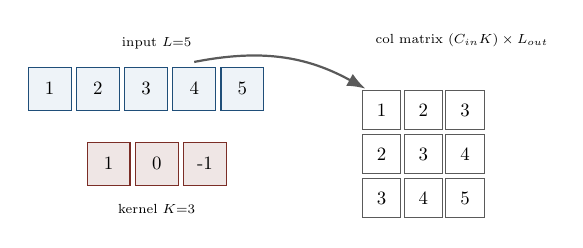
\begin{tikzpicture}[scale=0.68, every node/.style={transform shape}]
  % input strip
  \foreach \k/\v in {0/1,1/2,2/3,3/4,4/5}
    \node[draw=ferblue, fill=ferlight, minimum size=0.8cm] at (\k*0.9,0) {\v};
  \node at (2.0,0.85) {\scriptsize input $L{=}5$};
  % kernel
  \foreach \k/\v in {0/1,1/0,2/-1}
    \node[draw=fermaroon, fill=fermaroon!12, minimum size=0.8cm] at (2+\k*0.9-0.9,-1.4) {\v};
  \node at (2.0,-2.25) {\scriptsize kernel $K{=}3$};
  % col matrix
  \foreach \r/\vals in {0/{1,2,3},1/{2,3,4},2/{3,4,5}} {
    \foreach \c/\v [count=\i from 0] in \vals
      \node[draw=fergray, fill=white, minimum size=0.72cm] at (6.2+\i*0.78,-0.4-\r*0.82) {\v};
  }
  \node at (7.7,0.9) {\scriptsize col matrix $(C_{in}K) \times L_{out}$};
  % arrows windows -> columns
  \draw[-{Latex}, thick, fergray] (2.7,0.5) to[bend left=20] (5.9,0.0);
\end{tikzpicture}
\caption{im2col: each window position becomes one column. Zero-padding is
implicit --- the scratch is memset to zero and out-of-range taps are skipped.}
\label{fig:im2col}
\end{figure}

The mapping is a closed form: \texttt{dst[(ic*K + k)*Lout + p] = src[ic*L +
p*stride + k - pad]} for in-range positions. With the weight reshaped (as a
view, no copy) to $(C_{out}, C_{in}{\cdot}K)$, convolution collapses into one
\texttt{fe\_matmul(W, col, out)} per batch item.

Two honest footnotes: \texttt{fe\_conv1d} is the \emph{only} kernel allowed to
allocate --- it \texttt{malloc}s the im2col scratch per call and frees it after
(a documented exception to the hot-path rule); and it still prints an
unconditional debug trace on stderr, violating the kernels-never-log policy
pending cleanup.

\section{AVX2 Matrix Multiply --- \texttt{simd/}}

\subsection{Runtime Detection}

No compile-time \texttt{-march=native} gambling: the kernel asks the CPU.

\begin{lstlisting}[style=cstyle,caption={simd/matmul\_avx2.c --- CPUID leaf 7, EBX bit 5}]
bool fe_cpu_has_avx2(void) {
    unsigned int eax, ebx, ecx, edx;
    if (!__get_cpuid(0, &eax, &ebx, &ecx, &edx)) return false;
    if (eax < 7) return false;
    __cpuid_count(7, 0, eax, ebx, ecx, edx);
    return (ebx >> 5) & 1;         /* AVX2 feature bit */
}
\end{lstlisting}

\subsection{Tiling and the Microkernel}

The kernel tiles M in blocks of MC $=64$ and K in KC $=256$, packing both into
cache-friendly buffers, then sweeps columns eight at a time (NR $=8$ --- one AVX2
register). The microkernel holds a $64 \times 8$ accumulator tile in registers
(\texttt{\_\_m256 acc[64]}) and streams:

\begin{lstlisting}[style=cstyle]
b_row = _mm256_loadu_ps(&B_tile[k*NR]);        /* 8 floats          */
a_ik  = _mm256_set1_ps(A_tile[i*kc + k]);      /* broadcast scalar  */
acc[i]= _mm256_fmadd_ps(a_ik, b_row, acc[i]);  /* fused mul-add     */
\end{lstlisting}

Each FMMA does 8 multiply-adds per register per cycle; holding C in registers
across the whole kc-loop amortizes stores. Cross-tile accumulation works because
C is memset once and accumulators reload/store C between kc blocks.

\textbf{Remainder columns} ($N \bmod 8 \neq 0$) fall back to scalar arithmetic
over the packed tiles, so arbitrary N works despite header comments claiming a
multiple-of-8 requirement.

\subsection{Measured Result}

At $256^2$: naive $\approx$ GFLOPS baseline vs.\ AVX2 delivering a documented
$\sim$13.4$\times$ speedup (\texttt{bench\_avx2} prints the live ratio).
Equivalence checking compares against the scalar kernel with a deliberately
loose pass threshold (max abs error $< 1.0$) --- loose enough to never block,
tight enough to catch structural bugs, which reorder but never grossly distort.

\section{Memory Planner --- \texttt{planner/}}

Neural-network activations have stack-like lifetimes: once consumed, a tensor is
dead. Allocating each its own buffer wastes most memory. The planner proves how
little one buffer actually needs.

\subsection{Step 1: Lifetimes}

Walking execution order, each non-weight output tensor opens an interval
\texttt{\{first\_use, last\_use\}}; every subsequent read extends
\texttt{last\_use}. Sizes come from dtype $\times$ product(shape).

\subsection{Step 2: Greedy Best-Fit Reuse}

Process intervals in creation order. For each, search a free-slot pool for the
smallest slot that (a) was freed strictly before this tensor's birth
(\texttt{freed\_at < first\_use}) and (b) fits the 64-byte-aligned request. Hit?
Reuse the offset. Miss? Bump the high-water mark. Either way the interval then
contributes a slot freed at its own \texttt{last\_use}.

\begin{figure}[h]
\centering
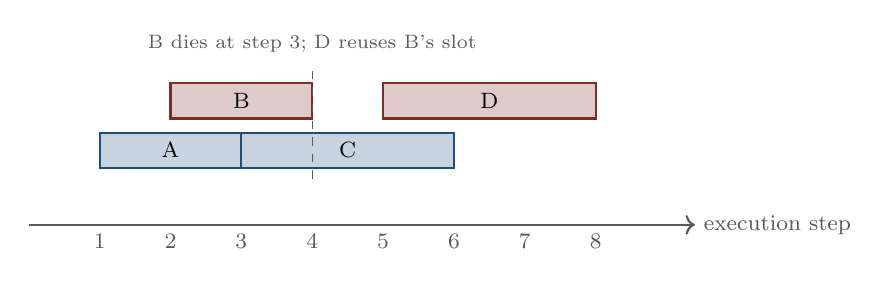
\begin{tikzpicture}[scale=0.9]
  \footnotesize
  % time axis
  \draw[->, thick, fergray] (0,-0.4) -- (9.4,-0.4) node[right] {execution step};
  \foreach \s in {1,...,8} \node[below, fergray] at (\s,-0.42) {\s};
  % intervals: (name, start, len, y, color)
  \foreach \nm/\st/\ln/\y/\cl in {A/1/2/0.4/ferblue, B/2/2/1.1/fermaroon,
                                  C/3/3/0.4/ferblue, D/5/3/1.1/fermaroon} {
    \fill[\cl!25, draw=\cl, thick] (\st,\y) rectangle ++(\ln,0.5);
    \node at ({\st+\ln/2},{\y+0.25}) {\nm};
  }
  \draw[dashed, fergray] (4,0.25) -- (4,1.8);
  \node[fergray, align=center, font=\scriptsize] at (4.0,2.15)
      {B dies at step 3; D reuses B's slot};
\end{tikzpicture}
\caption{Interval reuse: C shares A's band after A dies; D inherits B's slot.
Total footprint = max overlap, not sum of sizes.}
\label{fig:plan}
\end{figure}

This is greedy interval coloring: not optimal, $O(n^2)$, and perfectly adequate
--- \texttt{fe\_plan\_print} reports the savings percentage against naive
allocation. The plan exposes \texttt{total\_activation\_bytes} (the proven
minimum) plus per-tensor offsets.

\paragraph{Integration status.} \texttt{fe\_plan\_apply(g, plan, buf, size,
meta\_arena)} exists and is exercised by \texttt{test\_planner} (it verifies
tensor data lands inside the activation buffer), but \texttt{fe\_runtime\_run}
still uses the arena bump allocator directly. Wiring the two together is the
roadmap's Phase 1 item.

\section{Execution Engine --- \texttt{runtime/}}

\texttt{FeRuntime} binds three moving parts: the graph, the two arenas, and an
optional profiler.

\begin{lstlisting}[style=cstyle]
typedef struct {
    FeGraph   *graph;
    FeArena    weight_arena;      /* allocated once at load   */
    FeArena    activation_arena;  /* reset every inference    */
    FeProfiler *profiler;         /* NULL = untimed           */
} FeRuntime;
\end{lstlisting}

\subsection{One Inference, Seven Steps}

\texttt{fe\_runtime\_run(rt, input, output)}:

\begin{enumerate}[itemsep=1pt]
\item Reset the activation arena (O(1) --- rewind one pointer).
\item Detach every non-weight tensor (views into dead memory must not linger).
\item Bind the input at the \texttt{FE\_OP\_INPUT} node --- zero-copy, the
      caller's buffer \emph{is} the graph's input tensor.
\item Infer missing shapes: placeholder entries (shape \{0\}) get filled by
      walking the topo order applying per-op shape rules (conv1d's
      $L_{out}$ formula, flatten's $\{n, rest\}$, matmul's inner-dimension
      check-by-construction).
\item Bump-allocate remaining activations from the activation arena.
\item Walk \texttt{topo\_order}; dispatch each node through a switch. Unknown ops
      print \texttt{"unimplemented op"} and return \texttt{FE\_ERR\_SHAPE} ---
      loud, never silent.
\item Copy the result to the caller via \texttt{fe\_tensor\_copy} (memcpy fast
      path when both sides are contiguous).
\end{enumerate}

Dispatch details worth noting: \texttt{ADD} rides \texttt{fe\_bias\_add}'s
broadcast semantics; \texttt{CONV1D} passes its third input only when present
(bias-less convolutions legal); \texttt{BATCHNORM} falls into the default arm
and fails loudly --- enum exists, kernel does not yet. Profiler hooks wrap every
dispatch: \texttt{t0 = profiler ? now() : 0} before, record-after --- zero cost
when untimed.

\paragraph{Library ops versus the dispatch surface.} The Stage 2 math backend
is, as of this writing, a \emph{library}, not a graph feature. The ops enum
(\texttt{graph/graph.h}) still ends at \texttt{FE\_OP\_FLATTEN};
the engine switch still handles only the original nine cases, and
\texttt{FE\_OP\_ADD} remains the bias-add broadcast --- \emph{not}
\texttt{fe\_add}. No node can name \texttt{fe\_sum}, \texttt{fe\_mul}, or the
stability helpers yet; wiring them in is a graph-enum addition, an importer
attribute/plumbing step, and new dispatch cases. The kernel contract makes this
future work mechanical: every Stage 2 function already returns
\texttt{FeStatus}, validates shapes, and never allocates.

\section{ONNX Importer --- \texttt{importer/}}

ONNX models are protobuf messages. Ferrite refuses the protobuf library and
implements the wire format by hand --- roughly sixty lines of reader.

\subsection{Wire Format Primer}

Protobuf encodes \emph{tag = (field\_number << 3) | wire\_type} as a varint,
followed by the value:

\begin{itemize}[itemsep=1pt]
\item \textbf{Varint (type 0):} 7 bits per byte, little-endian groups, MSB =
      ``one more byte follows.''
\item \textbf{Length-delimited (type 2):} varint length, then that many bytes
      --- strings, sub-messages, raw tensors.
\item Types 1 and 5 are fixed 64/32-bit; the skipper handles all four so
      unknown fields cost nothing.
\end{itemize}

\begin{lstlisting}[style=cstyle,caption={importer/onnx.c --- the complete varint decoder}]
uint64_t fe_pb_varint(FePbReader *r) {
    uint64_t result = 0;  int shift = 0;
    while (r->pos < r->len) {
        unsigned char b = r->data[r->pos++];
        result |= (uint64_t)(b & 0x7F) << shift;
        if (!(b & 0x80)) return result;   /* MSB clear: last byte */
        shift += 7;
    }
    return 0;                             /* exhausted */
}
\end{lstlisting}

\subsection{What Gets Parsed}

Only the fields the engine needs; everything else flows through the generic
skipper:

\begin{table}[h]
\centering
\small
\begin{tabularx}{\textwidth}{@{}lllX@{}}
\toprule
\textbf{Message} & \textbf{Field} & \textbf{Name} & \textbf{Treatment} \\
\midrule
ModelProto & 7 & graph & length-delimited sub-message; everything else skipped\\
GraphProto & 1 & node & repeated NodeProto, in file order\\
GraphProto & 5 & initializer & weights; raw bytes memcpy'd into the weight arena\\
NodeProto & 1 & input & tensor name, resolved by linear name search\\
NodeProto & 2 & output & tensor name\\
NodeProto & 3 & name & node name used by the profiler report\\
NodeProto & 4 & op\_type & string mapped through the op table\\
NodeProto & 5 & attribute & sub-message: field 1 name, 7 ints (cap 8), 8 i\\
TensorProto & 1 & dims & repeated int64; $>$8 dims discarded\\
TensorProto & 9 & raw\_data & raw little-endian float32 payload\\
\bottomrule
\end{tabularx}
\caption{Parsed protobuf fields. Everything unparsed is skipped, never assumed.}
\end{table}

Attributes resolve to the graph union only where an op consumes them:
\texttt{pads} $\rightarrow$ \texttt{attrs.conv1d.pad},
\texttt{strides[0]} $\rightarrow$ stride, \texttt{kernel\_shape[0]} $\rightarrow$
kernel length. Softmax axis and Gemm coefficients are not extracted --- the
engine assumes defaults.

\begin{table}[h]
\centering
\begin{tabular}{@{}lll@{}}
\toprule
\textbf{ONNX string} & \textbf{FeOpType} & \textbf{Attribute notes} \\
\midrule
MatMul & MATMUL & --\\
Gemm & LINEAR & alpha/beta/transpose attrs are ignored\\
Relu & RELU & --\\
Softmax & SOFTMAX & axis attr is not extracted\\
Conv & CONV1D & pads[0..1], strides[0], kernel\_shape[0] parsed\\
BatchNormalization & BATCHNORM & loads but engine dispatch fails loudly\\
Add & ADD & mapped to the broadcast-bias kernel\\
Flatten & FLATTEN & --\\
\bottomrule
\end{tabular}
\caption{Op recognition map. Unknown strings print a warning and drop the node
--- the importer's one silent behavior, flagged as a roadmap fix.}
\end{table}

\subsection{Initializers Become Weights}

Each initializer's dims define the tensor entry; \texttt{is\_weight = 1}; raw
bytes are \texttt{memcpy}'d into a fresh 64-byte-aligned slot of the weight
arena. Names resolve through a linear registry search, creating placeholders
(shape \{0\}) for activations mentioned before definition --- placeholders are
what step 4 of the run loop fills in. After parsing: one topological sort, a
summary line, done. Limits mirror the graph caps (dims $\le 8$, names $\le 64$,
whole-file buffering).

Notably absent: \texttt{value\_info} parsing (external shape hints) and
\texttt{opset\_import} handling. Models must be built from supported ops with
inferable shapes.

\section{Quantization --- \texttt{quantization/}}

Symmetric per-tensor INT8: shrink weights 4$\times$, compute through integer
accumulate, accept bounded error.

\begin{align}
s &= \frac{\max_i |w_i|}{127}, \qquad q_i = \mathrm{clamp}\big(\mathrm{round}(w_i / s),\ -127,\ 127\big) \\
\hat w_i &= q_i \cdot s \qquad\qquad\text{(dequantize; zero point fixed at 0)}
\end{align}

Symmetry buys simplicity: no zero-point term anywhere, and the sign bit stays
meaningful. The scale floors at $10^{-8}$ so all-zero tensors never divide by
zero.

\texttt{fe\_matmul\_int8} quantizes both operands, accumulates in
\texttt{int32} (products of int8 need 16+ bits; summation needs headroom), then
rescales once:
$c_{ij} = \text{acc}_{ij} \cdot s_A \cdot s_B$.

\begin{lstlisting}[style=cstyle]
int32_t acc = 0;
for (int k = 0; k < K; k++)
    acc += (int32_t)a_q[i*K+k] * (int32_t)b_q[k*N+j];
float out_scale = pA.scale * pB.scale;
c[i*N+j] = (float)acc * out_scale;
\end{lstlisting}

Measured in \texttt{test\_quant}: endpoint codes hit exactly $\pm 127$,
dequantization error stays under $0.05$, int8-GEMM error under $0.1$ versus
float32, and int8 payloads are asserted \emph{exactly} 75\% smaller than f32.
Per-channel scales (per output row) would tighten accuracy further --- deferred
deliberately.

\section{Profiler, Benchmarks, Demo --- \texttt{tools/}}

\texttt{FeProfiler} accumulates \{name, total\_ns, calls\} records keyed by node
name (linear search, cap 64 distinct ops). The clock is
\texttt{clock\_gettime(CLOCK\_MONOTONIC)} folded to nanoseconds --- wall time
immune to frequency scaling artifacts across cores. Reports insertion-sort
descending by total and print Calls / Total / Avg / \% Time, ending with a TOTAL
row: the hotspot table is always one call away.

Two benchmark harnesses share methodology (N $=$ 256, one warmup, 20 timed
runs, GFLOPS $= 2N^3 / \text{ms} / 10^6$): \texttt{bench\_matmul} baselines the
scalar kernel; \texttt{bench\_avx2} additionally refuses to run without CPUID
support, verifies against the scalar oracle, and prints the speedup ratio.

The end-to-end demo (\texttt{demo}) loads a real 1-D CNN ONNX model for acoustic
pipe-leak detection (\texttt{acousticleaknet.onnx}), synthesizes one second of
composite sine audio at 8 kHz, classifies it into \{No Leak, Small Leak, Large
Leak\}, renders ASCII probability bars, sanity-checks the softmax sum within
$10^{-3}$, averages five timed runs, and prints the profiler table plus
weight/peak-activation megabytes.

\section{Tests and Build System}

\subsection{Build Story}

CMake is canonical: one command configures, builds all test binaries, and
registers them with CTest. Per-subsystem static libraries make the layer rule
mechanical --- a downward dependency violation is a link error. Sanitizer
support (ASan + UBSan) is \emph{probed} at configure time: toolchains shipping
the runtimes get instrumented binaries; others degrade with a status message
rather than failing. On Windows/MinGW each executable copies the matching
\texttt{libwinpthread-1.dll} beside itself, defeating stale DLL copies found on
PATH. Requires GCC/Clang (the POSIX clock excludes MSVC).

\paragraph{Build-system drift (a real incident).} The Stage 2 commit wired the
three new sources into the \emph{Makefile} (its \texttt{test\_ops} rule gained
\texttt{ops/elementwise.o ops/reduce.o ops/stability.o}, plus dependency rules),
but \emph{not} into CMake: the committed \texttt{ferrite\_ops} target listed
only matmul/activations/conv1d, so a CMake build of \texttt{test\_ops} failed
to link with undefined \texttt{fe\_add}/\texttt{fe\_div}/\texttt{fe\_sum}
symbols. The fix --- adding the three sources to \texttt{ferrite\_ops} --- is
required for Windows/MinGW development. The same commit also exposed a Makefile
typo: the pre-existing \texttt{ops/matmul.o} rule wrote to
\texttt{-o ops/matmul.} (trailing dot), which on Linux silently produced an
ELF object named \texttt{ops/matmul.} --- which was then committed as a
``source'' file. On Windows that name is impossible to check out
(trailing-dot paths fail NTFS validation), and the stray binary was deleted;
the Makefile line remains a genuine typo to fix upstream.

\subsection{Test Inventory}

One binary per subsystem, each asserting invariants under sanitizers:

\begin{table}[h]
\centering
\small
\begin{tabularx}{\textwidth}{@{}l X@{}}
\toprule
\textbf{Target} & \textbf{Asserts} \\
\midrule
test\_tensor & strided ops, reshape/transpose/contiguous repack; slice views; stride-0 broadcast \{1,3\}-$>$\{4,3\}; allclose tolerances\\
test\_allocator & arena alignment math, reset identity, exhaustion, arena tensors\\
test\_ops & matmul identity + known [[1,2],[3,4]]@[[5,6],[7,8]]=[[19,22],[43,50]]; relu; softmax sums to 1, stable on \{1000,1e3,1002\}; elementwise add/mul/div exact; mul\_scalar/neg; axis sum/max on \{2,3\}; dot=32; logsumexp in (1000,1003)\\
test\_graph & linear-chain topo order; diamond graph fan-out / merge\\
test\_engine & 1-4-8-3 MLP, uniform 0.1 weights =$>$ every softmax output exactly 1/3\\
test\_onnx & loads tests/tiny\_mlp.onnx; topo valid; weight arena non-empty\\
test\_planner & reuse beats naive byte total; fe\_plan\_apply pointer placement\\
test\_conv1d & edge detector \{1,0,-1\}, multichannel all-ones, pad=1 sum filter\\
test\_profiler & MLP under profiler, 10 runs, sorted report printed\\
test\_quant & scale == 1/127, endpoints +-127, dequant $<$ 0.05, matmul err $<$ 0.1, exactly 75\% smaller\\
test\_tensor\_ser & round-trips (all dtypes, up to 8-D), view saves canonical, 8 corruption cases\\
\bottomrule
\end{tabularx}
\caption{Test targets. The engine test's uniform-weight MLP produces logits so
similar that softmax must yield exactly 1/3 per class --- a sharp, cheap
end-to-end oracle.}
\end{table}

\section{End-to-End Flow}

Tracing one inference through every layer:

\begin{center}
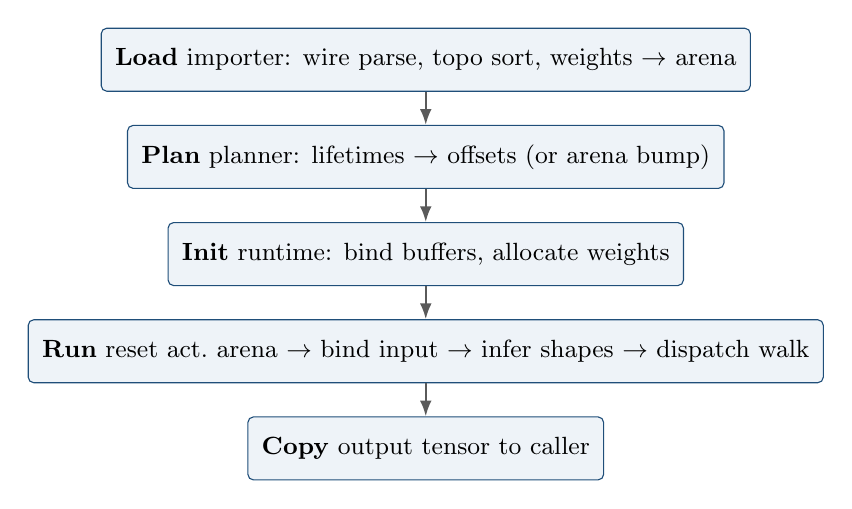
\begin{tikzpicture}[node distance=0.42cm,
  box/.style={rectangle, rounded corners=2pt, draw=ferblue, fill=ferlight,
              minimum height=0.8cm, inner sep=5pt, font=\small},
  arr/.style={-{Latex[length=2mm]}, thick, fergray}]
  \node[box] (load) {\textbf{Load} importer: wire parse, topo sort, weights $\to$ arena};
  \node[box, below=of load] (plan) {\textbf{Plan} planner: lifetimes $\to$ offsets (or arena bump)};
  \node[box, below=of plan] (init) {\textbf{Init} runtime: bind buffers, allocate weights};
  \node[box, below=of init] (run) {\textbf{Run} reset act.\ arena $\to$ bind input $\to$ infer shapes $\to$ dispatch walk};
  \node[box, below=of run] (copy) {\textbf{Copy} output tensor to caller};
  \draw[arr] (load) -- (plan);
  \draw[arr] (plan) -- (init);
  \draw[arr] (init) -- (run);
  \draw[arr] (run) -- (copy);
\end{tikzpicture}
\end{center}

Concretely, \texttt{tiny\_mlp.onnx} exercises the whole chain: protobuf fields
resolve to MATMUL/RELU/MATMUL/SOFTMAX nodes; initializer bytes land aligned in
the weight arena; Kahn's algorithm orders five nodes; uniform $0.1$ weights make
every logit identical, so the softmax output must equal exactly $1/3$ per class
--- the number \texttt{test\_engine} asserts.

\section{Known Limitations, Honestly}
\label{sec:honest}

\begin{itemize}[itemsep=2pt]
\item \textbf{Stage 2 is library-only.} \texttt{fe\_add}/\texttt{fe\_sum}/
      \texttt{fe\_logsumexp} \& co.\ have no \texttt{FE\_OP\_*} enum values and
      no dispatch cases; the engine switch still stops at \texttt{FLATTEN} and
      \texttt{FE\_OP\_ADD} still means bias-add.
\item \textbf{Elementwise kernels are contiguous-only.} They index flat and
      ignore strides, so a stride-0 broadcast view misfeeds them; reduce and
      stability read strided and are view-correct. A shared strided walker
      would close the gap.
\item \textbf{Test gaps in the math layer:} \texttt{fe\_sub},
      \texttt{fe\_add\_scalar}, \texttt{fe\_sub\_scalar}, \texttt{fe\_div\_scalar},
      and \texttt{fe\_min} have no direct assertions, and no broadcast view is
      ever pushed through an op.
\item \textbf{Planner unwired.} \texttt{fe\_plan\_apply} is tested standalone
      but the runtime still bump-allocates. Roadmap Phase 1.
\item \textbf{BATCHNORM has no kernel.} Loads fine; dispatch fails loudly with
      \texttt{FE\_ERR\_SHAPE}.
\item \textbf{Unsupported ONNX ops are dropped with a warning}, not rejected.
      Should be a hard error.
\item \textbf{No shape inference from \texttt{value\_info}}; no opset handling.
      Models must fit the supported subset with inferable shapes.
\item \textbf{Per-tensor quantization only}; per-channel scales would help
      accuracy on outlier channels.
\item \textbf{\texttt{fe\_conv1d} violates two policies}: per-call scratch
      \texttt{malloc} (documented exception) and an unconditional debug
      \texttt{fprintf} (undocumented; pending removal).
\item \textbf{Declared-but-unimplemented}: \texttt{fe\_quantize\_weights} exists
      only as a prototype.
\item \textbf{Single-threaded}; fixed capacities (512/1024/8); AVX2 remainder
      columns run scalar.
\item \textbf{Cross-platform:} Windows pulls need \texttt{core.protectntfs=false}
      until the stray \texttt{ops/matmul.} binary is purged upstream, and the
      CMake \texttt{ferrite\_ops} source list must stay in sync with the
      Makefile.
\end{itemize}

\subsection{Source File Index}


\begin{tabularx}{\textwidth}{@{}l X@{}}
\toprule
\textbf{File(s)} & \textbf{Role} \\
\midrule
core/types.h & FeDtype, FeStatus enums, fe\_dtype\_size, FERRITE\_MAX\_DIMS=8 \\
core/tensor.c/h & FeTensor strided views: alloc/slice/transpose/reshape/contiguous/copy; stride-0 broadcast\_to; numel; get/set\_f32; allclose \\
core/tensor\_ser.c/h & versioned binary serialization (FETN v1), strict validating reader \\
core/allocator.c/h & FeArena bump allocator; pointer-address alignment; peak tracking \\
core/log.c/h & fe\_log level-filtered stderr logging (compile-time minimum) \\
graph/graph.c/h & fixed-capacity IR: nodes, tensor registry, Kahn topological sort \\
ops/matmul.c & i-k-j scalar reference + AVX2 dispatch behind CPUID gate; fe\_linear wrapper \\
ops/activations.c & relu, last-axis stable softmax (inv-sum third pass), broadcast bias\_add \\
ops/elementwise.c & fe\_add/sub/mul/div + scalar variants + fe\_neg; exact-shape fp32 flat loops \\
ops/reduce.c & single-axis fe\_sum/fe\_max/fe\_min with axis-removed output; rank-1 fe\_dot \\
ops/stability.c & max-shift fe\_logsumexp and fe\_stable\_exp\_normalize (1-D fp32, two passes) \\
ops/conv1d.c & im2col transformation + matmul; per-call scratch buffer \\
simd/matmul\_avx2.c/h & tiled AVX2+FMA microkernel; CPUID detection; remainder columns \\
planner/memory\_planner.c/h & lifetime analysis + greedy best-fit buffer reuse; FePlan offsets \\
runtime/engine.c/h & FeRuntime lifecycle, shape inference, dispatch walk, output copy \\
importer/onnx.c & hand-written protobuf wire parser -$>$ graph build -$>$ weights to arena \\
quantization/quant.c & symmetric INT8 per-tensor quantize/dequantize + int8 GEMM path \\
tools/profiler.c & per-op ns timing records, CLOCK\_MONOTONIC, sorted report \\
tools/bench\_matmul.c & naive GFLOPS at N=256 over 20 runs \\
tools/bench\_avx2.c & AVX2 vs naive GFLOPS, correctness verify, speedup print \\
tools/demo\_acousticleaknet.c & end-to-end demo: acoustic leak-detection CNN on synthetic audio \\
\bottomrule
\end{tabularx}


\vfill
\begin{center}
\color{fergray}\rule{0.6\textwidth}{0.4pt}\\[4pt]
\small Generated by \texttt{temps/build\_guide.py} --- edit the script, rerun,
and this document rebuilds itself.
\end{center}

\end{document}
